% mnras_template.tex 
%
% LaTeX template for creating an MNRAS paper
%
% v3.0 released 14 May 2015
% (version numbers match those of mnras.cls)
%
% Copyright (C) Royal Astronomical Society 2015
% Authors:
% Keith T. Smith (Royal Astronomical Society)

% Change log
%
% v3.0 May 2015
%    Renamed to match the new package name
%    Version number matches mnras.cls
%    A few minor tweaks to wording
% v1.0 September 2013
%    Beta testing only - never publicly released
%    First version: a simple (ish) template for creating an MNRAS paper

%%%%%%%%%%%%%%%%%%%%%%%%%%%%%%%%%%%%%%%%%%%%%%%%%%
% Basic setup. Most papers should leave these options alone.
\documentclass[fleqn,usenatbib]{mnras}

% MNRAS is set in Times font. If you don't have this installed (most LaTeX
% installations will be fine) or prefer the old Computer Modern fonts, comment
% out the following line
\usepackage{newtxtext,newtxmath}
% Depending on your LaTeX fonts installation, you might get better results with one of these:
%\usepackage{mathptmx}
%\usepackage{txfonts}

% Use vector fonts, so it zooms properly in on-screen viewing software
% Don't change these lines unless you know what you are doing
\usepackage[T1]{fontenc}
\usepackage{ae,aecompl}


%%%%% AUTHORS - PLACE YOUR OWN PACKAGES HERE %%%%%

% Only include extra packages if you really need them. Common packages are:
\usepackage{graphicx}	% Including figure files
\usepackage{amsmath}	% Advanced maths commands
\usepackage{amssymb}	% Extra maths symbols

%%%%%%%%%%%%%%%%%%%%%%%%%%%%%%%%%%%%%%%%%%%%%%%%%%

%%%%% AUTHORS - PLACE YOUR OWN COMMANDS HERE %%%%%

% Please keep new commands to a minimum, and use \newcommand not \def to avoid
% overwriting existing commands. Example:
%\newcommand{\pcm}{\,cm$^{-2}$}	% per cm-squared

%%%%%%%%%%%%%%%%%%%%%%%%%%%%%%%%%%%%%%%%%%%%%%%%%%

%%%%%%%%%%%%%%%%%%% TITLE PAGE %%%%%%%%%%%%%%%%%%%

% Title of the paper, and the short title which is used in the headers.
% Keep the title short and informative.
\title{Gas Fractions of Galaxies Across Simulations}

% The list of authors, and the short list which is used in the headers.
% If you need two or more lines of authors, add an extra line using \newauthor
\author[Emerick]{ Andrew Emerick$^{1,2}$\thanks{E-mail: emerick@astro.columbia.edu} + more + IQ Collaboratory (alphabetical order)
\\
% List of institutions
$^{1}$Department of Astronomy, Columbia University, New York, NY 10027 \\
$^{2}$Department of Astrophysics, American Museum of Natural History, New York, NY
}

% These dates will be filled out by the publisher
\date{Accepted XXX. Received YYY; in original form ZZZ}

% Enter the current year, for the copyright statements etc.
\pubyear{2015}

% Don't change these lines
\begin{document}
\label{firstpage}
\pagerange{\pageref{firstpage}--\pageref{lastpage}}
\maketitle

% Abstract of the paper
\begin{abstract}
{\bf NOTE: all plots should be considered preliminary for both style and content}
\end{abstract}

% Select between one and six entries from the list of approved keywords.
% Don't make up new ones.
\begin{keywords}
keyword1 -- keyword2 -- keyword3
\end{keywords}

%%%%%%%%%%%%%%%%%%%%%%%%%%%%%%%%%%%%%%%%%%%%%%%%%%

%%%%%%%%%%%%%%%%% BODY OF PAPER %%%%%%%%%%%%%%%%%%

\section{Introduction}



Modern large cosmological hydrodynamics simulations have made tremendous progress in being able to reproduce observed properties of galaxies. This progress is fueled both by better computational resources, allowing for increased dynamic range in these simulations, and more careful attention to models of feedback. Updated sub-grid methods for stellar feedback physics better describe how feedback regulates star formation and drives outflows in galaxies. To obtain these improvements, however, the free many parameters associated with these models are generally calibrated specifically to reproduce observed relationships of the stellar properties galaxies, such as the galaxy stellar mass function (GSFMS), the stellar mass halo mass (SMHM) relationship, galaxy sizes, and/or the redshift evolution of these relations. Understanding how well, if at all, a given simulation that reproduces galaxy stellar properties matches galaxy gas properties is an important tool to better understand the physics that drives galaxy evolution. The differences among these models are significant enough that, even with similar galaxy stellar mass properties, galaxy gas properties are not necessarily comparable. Although this study has been done individually for EAGLE \citep{Bahe2016,Marasco2016,Crain2017}, MUFASA \citep{Dave2017}, (and {\it Illustris + SAM?}), these works have never been compared with each other simultaneously. In this work we examine the gas properties of galaxies between Illustris \citep{Vogelsberger2014,Genel2014}, EAGLE \citep{Schaye2015,Crain2015}, MUFASA \citep{Dave2016}, and the ``Santa Cruz'' SAM \citep{Somerville2012,Porter2014} {\it check these refs.}.

% Illustris TNG??

\section{Simulations and Data Selection}
\begin{table*}
\centering
\caption{Caption}
\label{table:simulations}
  \begin{tabular}{l c c c c c c c}
  \hline
  Simulation & Baryon Res. (10$^6$ M$_{\odot}$) & DM Res. (10$^6$ M$_{\odot}$) & Vol. (x cMpc)$^3$ & $\epsilon$ (ckpc) & Gas Def. & Pressure Floor & Ref. \\
  \hline 
  Illustris  & 1.26 ($\Delta x$ = 48 cpc) & 6.26 & 106.5 & 0.71 / 1.42 & &  & \citep{Vogelsberger2014} \\
  %Illustris-TNG & & & \\
  MUFASA & 18.2 & 96 & 50 & 0.5 & & & \citep{Dave2016} \\
  EAGLE  & 1.81 &  9.70  & 100 & 0.70 (pkpc) & &  & \citep{Schaye2015,Crain2015} \\
  SC-SAM & -  & - & & - & - & & \citep{Somerville2012,Porter2014}\\
  \hline
  \end{tabular}
  
\end{table*}

For each data source we utilize all central galaxies, as determined by a halo finder, without consideration of nearest-neighbor distance to a comparably massive or more massive galaxy. {\it (list halo finders used across simulations for clarity? Likely not the same)}. We consider all gas, stellar, and dark matter mass assigned as belonging to the central galaxy by the halo finder, ignoring mass assigned to sub-halos. In truth, this selection can include a large amount of gas in the circumgalactic medium (CGM), far from the central galaxy. However, we focus our attention solely on the cold gas content of these galaxies, which should be be contained predominately in the disk of the galaxy. SFR's and sSFR's are computed as averaged over 100~Myr and 1~Gyr.

The works considered here treat the sub-grid physics required to model individual gas components (e.g. H, He, H$_2$) and their ionization states somewhat differently. Each of the big-box simulations lack the resolution and physics needed to self-consistently model each ionization state. Rather, these are computed through some approximation either live during the simulation (EAGLE) or via post-processing (MUFASA). Though each of these methods are similar, they likely do not produce identical results; characterizing the variation in galaxy gas properties caused by different ionization models is beyond the scope of this work. If H$_2$ is followed, we compute the gas mass of each galaxy as the total neutral hydrogen mass, or M$_{\rm gas}$ = M$_{\rm H_2}$ + M$_{\rm \ion{H}{i}}$ (EAGLE, MUFASA), otherwise we take M$_{\rm gas}$ = M$_{\rm \ion{H}{i}}$ if H$_2$ is not tracked (Illustris, SC-SAM). This is a more faithful comparison than taking M$_{\rm \ion{H}{i}}$ alone, as the H$_2$ content in these works is derived directly from the \ion{H}{i} content. We define gas fraction here as
\begin{equation}
f_{\rm gas} = \frac{M_{\rm HI}}{M_{\rm HI} + M_{*}},
\end{equation}
though we note some authors consider instead the the ratio $M_{\ion{H}{i}} / M_{*}$.

We briefly describe each data source below including how gas phases are computed for each work. We refer the reader to the individual method papers associated with these works for detailed descriptions. The properties of these simulations are summarized in Table~\ref{table:simulations}.

{\bf For each of the below need: 1) code + hydro (SPH, moving mesh, etc.), 2) included feedback physics and briefly how they are modeled (thermal? mechanical? any hydro or cooling decoupling? AGN threshold / methods if they exist, etc.), 3) brief characterization of the feedback physics (bursty, strong, weak, etc.), 4) how is neutral gas followed / computed in each work, and 5) resolution and box size.}
\subsection{Illustris}
\label{sec:illustris method}
{\it ask Shy for text}

\subsection{EAGLE}
\label{sec:EAGLE method}
{\it ask ?? for text}

\subsection{MUFASA}
\label{sec:MUFASA method}
{\it ask Romeel for text}

\subsection{SC SAM}
\label{sec:SC-SAM method}
{\it ask Rachel and/or Viraj for text}

\subsection{Observational datasets}
\label{sec:observational data}
{\bf decide if we are making observational comparisons.} describe datasets here ({\it Marla for text?}).. likely both Bradford et. al. 2015 and recent xGASS data release.

\section{Results}
\label{sec:results}
%\subsection{Gas mass vs stellar mass}
%Maybe just ignore this for simplicity in favor of gas fraction plots

\subsection{Stellar Mass Halo Mass Relationship}
\label{sec:results:SMHM}
{\it Discuss SMHM relationship across data with references to original publications. Main story: Stellar properties of galaxies are similar (this is one example). Physics that generates these similar properties is very different. Leads into how this may affect related but un-tuned properties (i.e. gas).}

\begin{figure*}
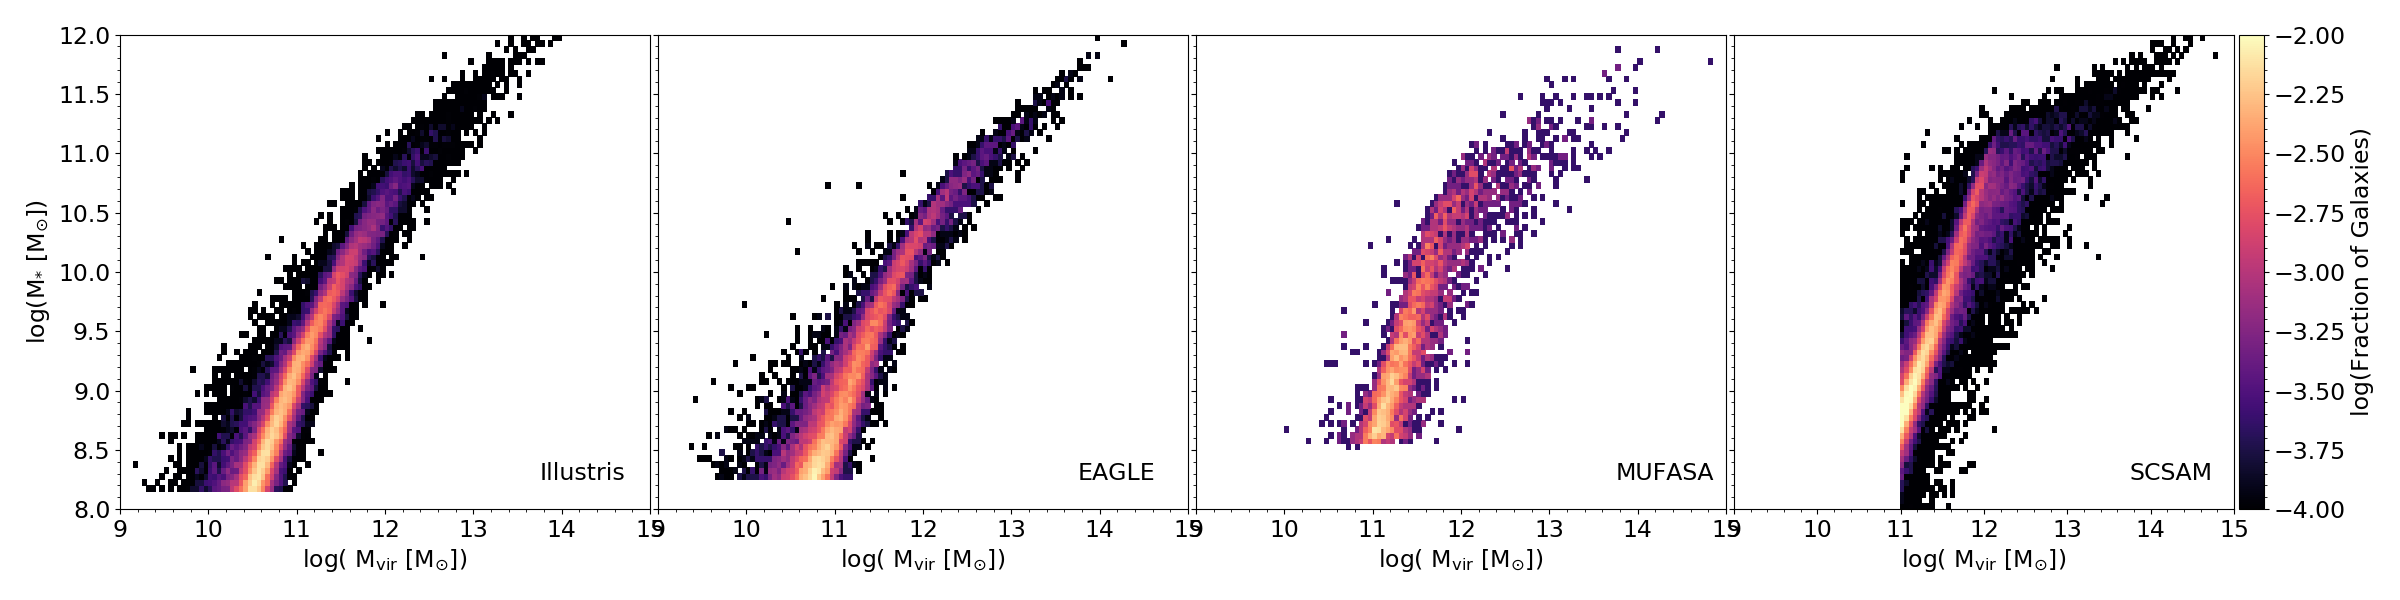
\includegraphics[width = 0.975\textwidth]{halo_stellar_2D_fraction.png}
\caption{The stellar mass halo mass relationship for the full population of galaxies across datasets. Shading indicates the fraction of galaxies within a given bin.}
\label{fig:fgas mstar 2D}
\end{figure*}


\subsection{Gas Fraction and Gas Mass vs stellar mass}
\label{sec:results:fg Mstar}

\begin{figure*}
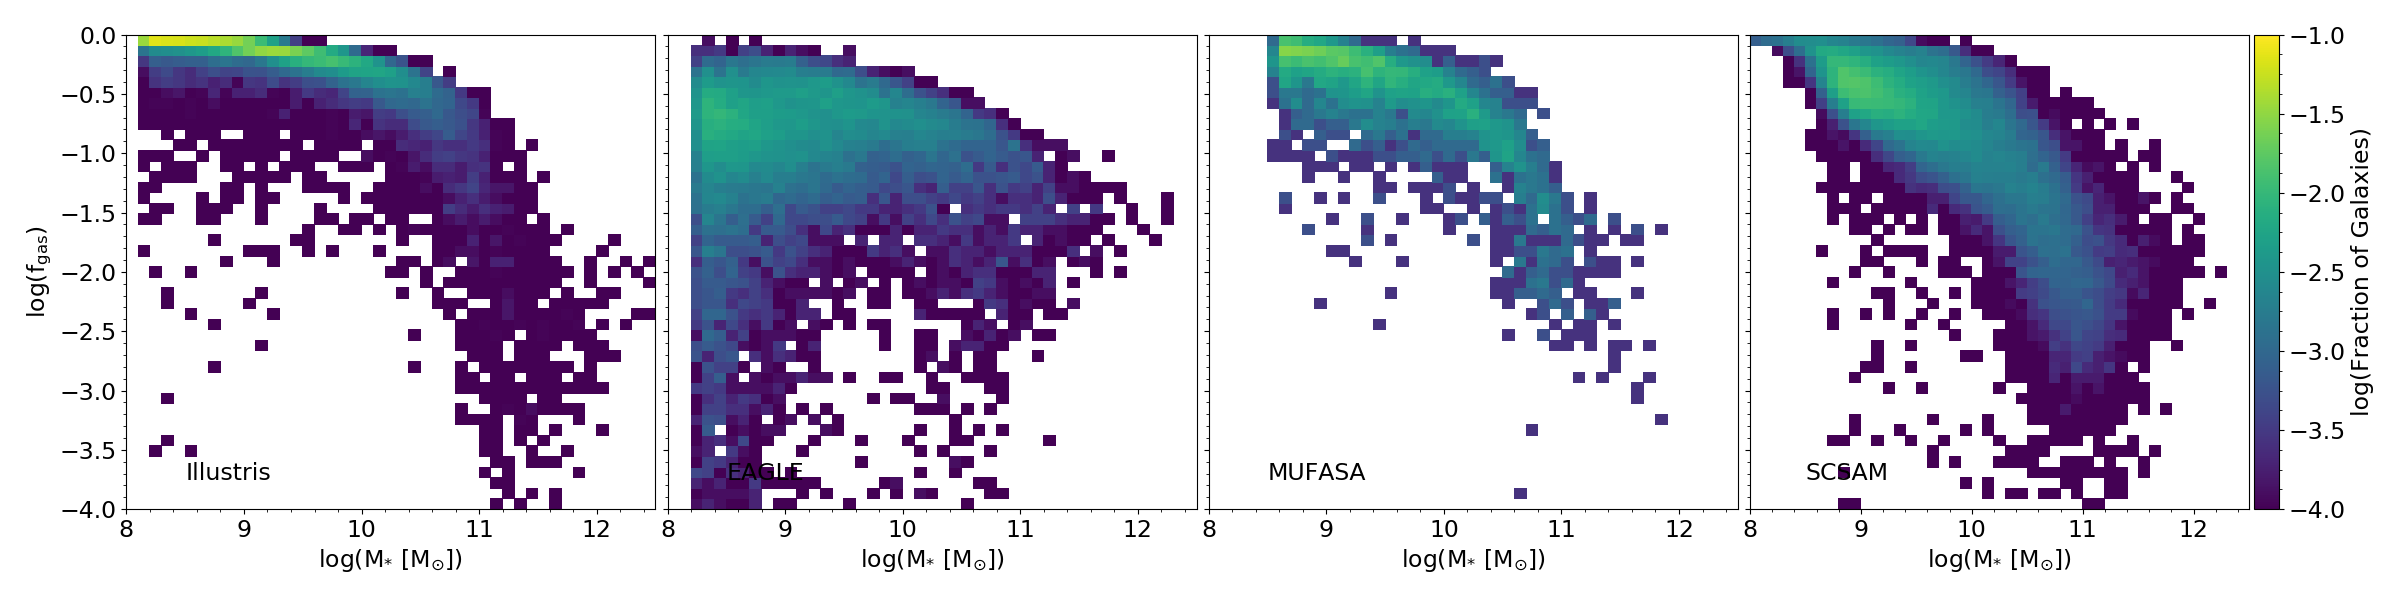
\includegraphics[width = 0.99\textwidth]{fgas_mstar_2D_log_fgas.png}
\caption{Galaxy gas fraction (f$_{\rm gas}$) as a function of stellar mass for the full population of galaxies in each of the four data sets with large galaxy counts. Shading indicates the fraction of galaxies in a given bin. This diagram explicitly does not include galaxies with f$_{\rm gas}$ = 0 (see Figure~\ref{fig:linear fgas mstar}).}
\label{fig:fgas mstar 2D}
\end{figure*}

In Figure~\ref{fig:fgas mstar 2D} we present the gas fraction as a function of stellar mass for the entire population of galaxies in each of the large sample-size datasets. To zeroth order, each data set has the same trend of decreasing gas fraction with increasing stellar mass, but the distribution of gas fractions at fixed stellar mass varies significantly across each data source. In particular, Illustris is more tightly distributed around high gas fractions than the other datasets, while the remaining have wider distributions and lower typical gas fractions. EAGLE exhibits the largest spread in gas fraction at fixed stellar mass. 

By nature of plotting gas fraction in logsapce, these diagrams exclude any galaxies with no gas content. To help clarify these populations across datasets we plot the median gas fraction (including galaxies with f$_{\rm gas}$ = 0) as a function of stellar mass in the top panel of Figure~\ref{fig:linear fgas mstar}. The shaded regions in each encompass the innerquartile range of each distribution; in stellar mass bins with less than 10 galaxies we plot points instead of the median curve. In the bottom panel, we show the fraction of galaxies in stellar mass bins that are devoid of gas for each data source. The same trends observed in Figure~\ref{fig:fgas mstar 2D} are clear here as well: Illustris galaxies are tightly distributed with high gas fractions at fixed stellar mass, as compared to EAGLE, MUFASA, and the SC-SAM which have comparable gas fractions and wider distributions. At low stellar mass, the SC-SAM approaches unity, unlike MUFASA and EAGLE. 

The bottom panel of Figure~\ref{fig:linear fgas mstar} is striking. This shows the fraction of galaxies in each stellar mass bin that contain no cold gas (defined again as either \ion{H}{i} or \ion{H}{i} and H$_2$), with the total percentage of gasless galaxies in each sample given in the legend. Both EAGLE and MUFASA uniformly have large populations of gasless galaxies across all stellar masses, with particularly high fractions at low stellar masses. In contrast, Illustris uniformly has very few galaxies devoid of cold gas at all stellar masses. The SC-SAM is the only model that evolves with stellar mass in this space. 

\begin{figure*}
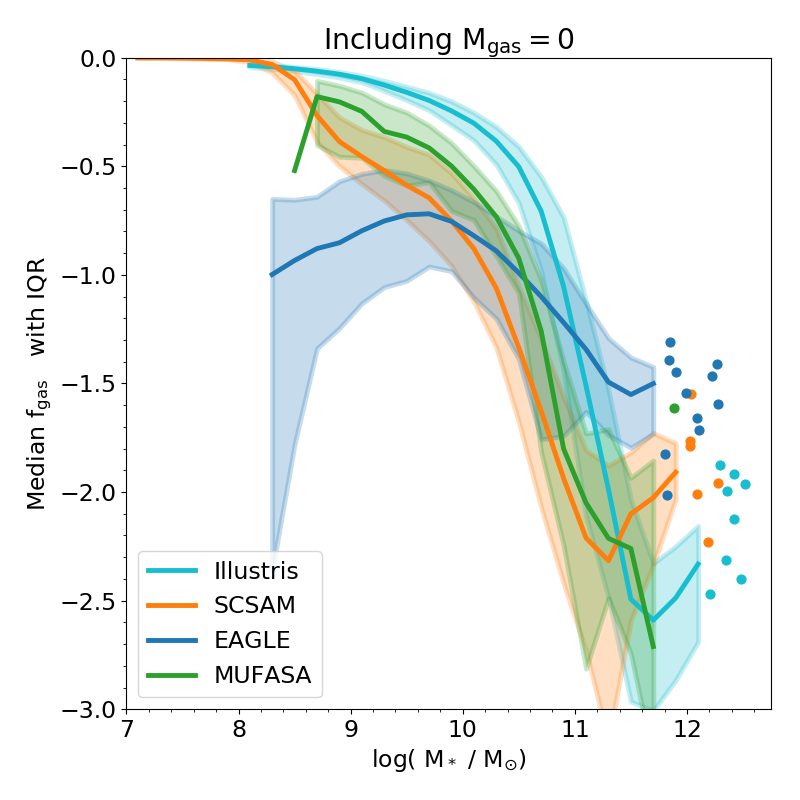
\includegraphics[width = 0.3\linewidth]{fgas_mstar_binned_IQR_logged.png}
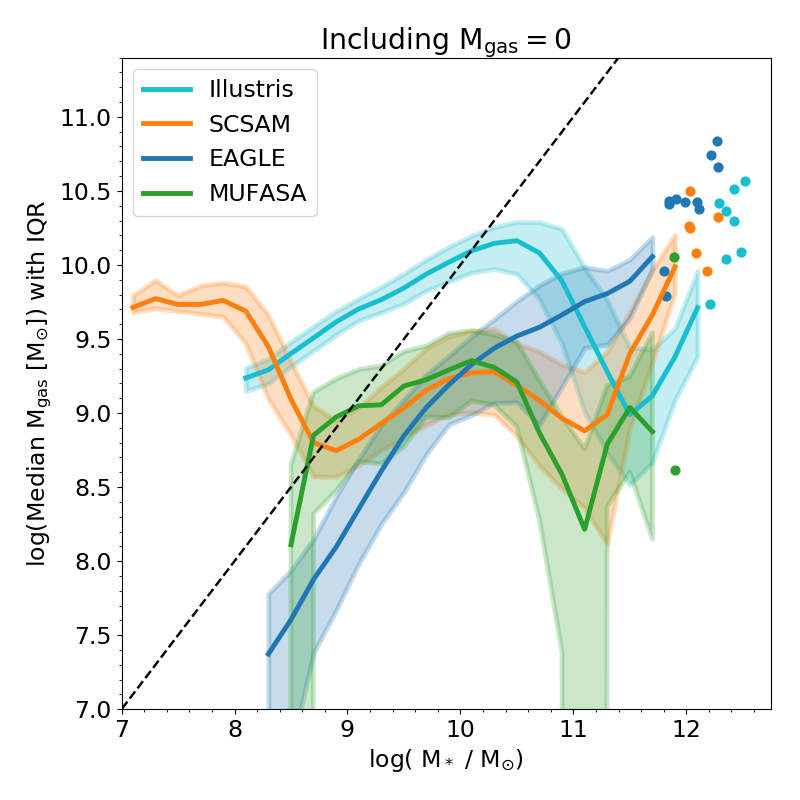
\includegraphics[width = 0.3\linewidth]{MHI_Mstar_binned_IQR.png}
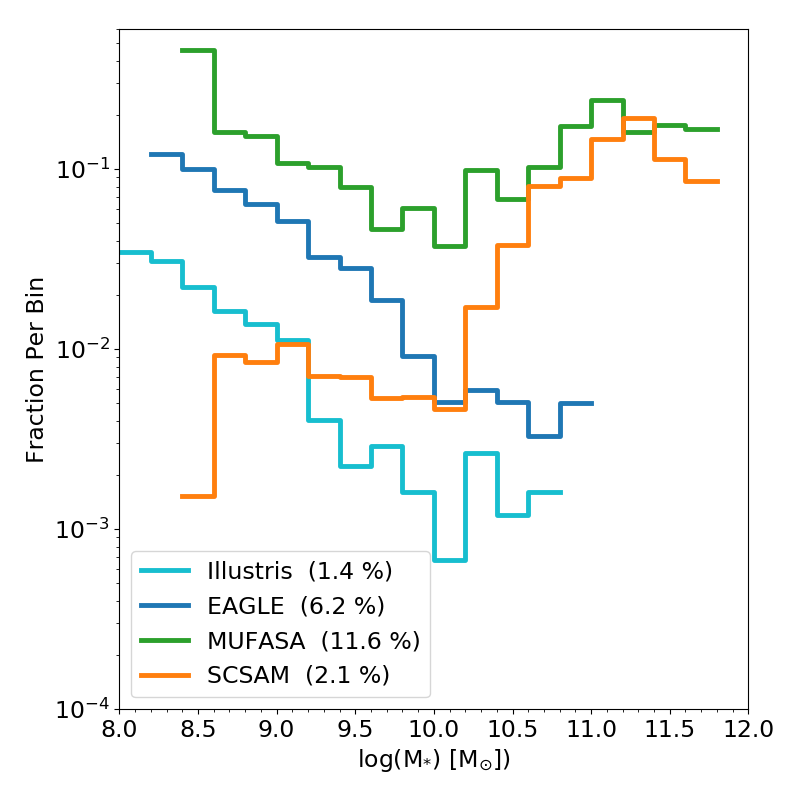
\includegraphics[width = 0.3\linewidth]{gasless_fraction_mstar.png}
\caption{{\bf Left:} The running median of f$_{\rm gas}$ as a function of stellar mass for each dataset with shading denoting the inner quartile range of each. Unlike in Figure~\ref{fig:fgas mstar 2D}, this includes galaxies with zero neutral gas mass. {\bf Middle} The running median of gas mass as a function of stellar mass for each dataset with shading denoting the IQR. {\bf Right:} The fraction of galaxies per stellar mass bin for each dataset that do not contain any neutral gas. The percent of all galaxies without gas in each dataset is shown in the legend.}
\label{fig:linear fgas mstar}
\end{figure*}

\subsection{SFR vs. stellar mass}
\label{sec:results:SFMS fgas}

\textit{ Establish definition of SFMS from Paper I. Discuss Figure~\ref{fig:SFMS fgas}. 
\begin{enumerate}
\item Significant variation among simulations as to where (relative to SFMS) galaxies are gas-rich and gas-poor.
\item SFMS slope is somewhat correlated with EAGLE f$_{\rm gas}$ = 0.5 line. Is this significant? Should they be related?
\item SCSAM galaxies at low stellar masses are gas rich above and below SFMS.
\end{enumerate}
}

\subsubsection{Distance from the main sequence and gas properties}
\label{sec:distance SFMS}

\begin{figure*}
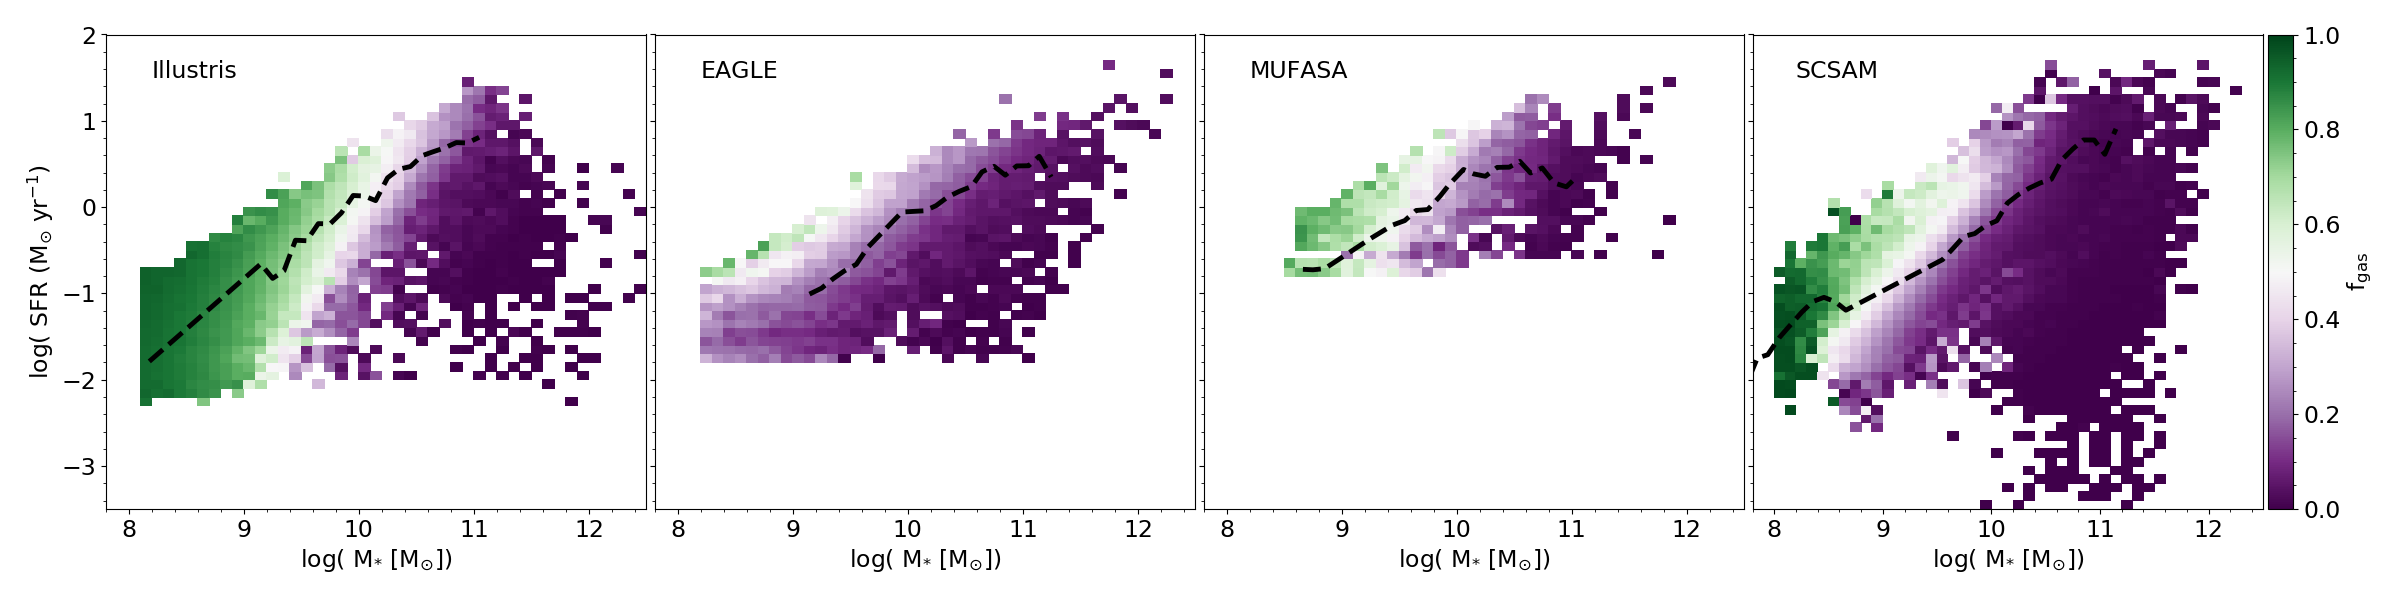
\includegraphics[width = 0.99\linewidth]{SFMS_fits_2dhist_median.png}\\
\caption{2D Histograms of the SFMS, colored by median gas fraction. }
\label{fig:SFMS fgas}
\end{figure*}

\begin{figure*}
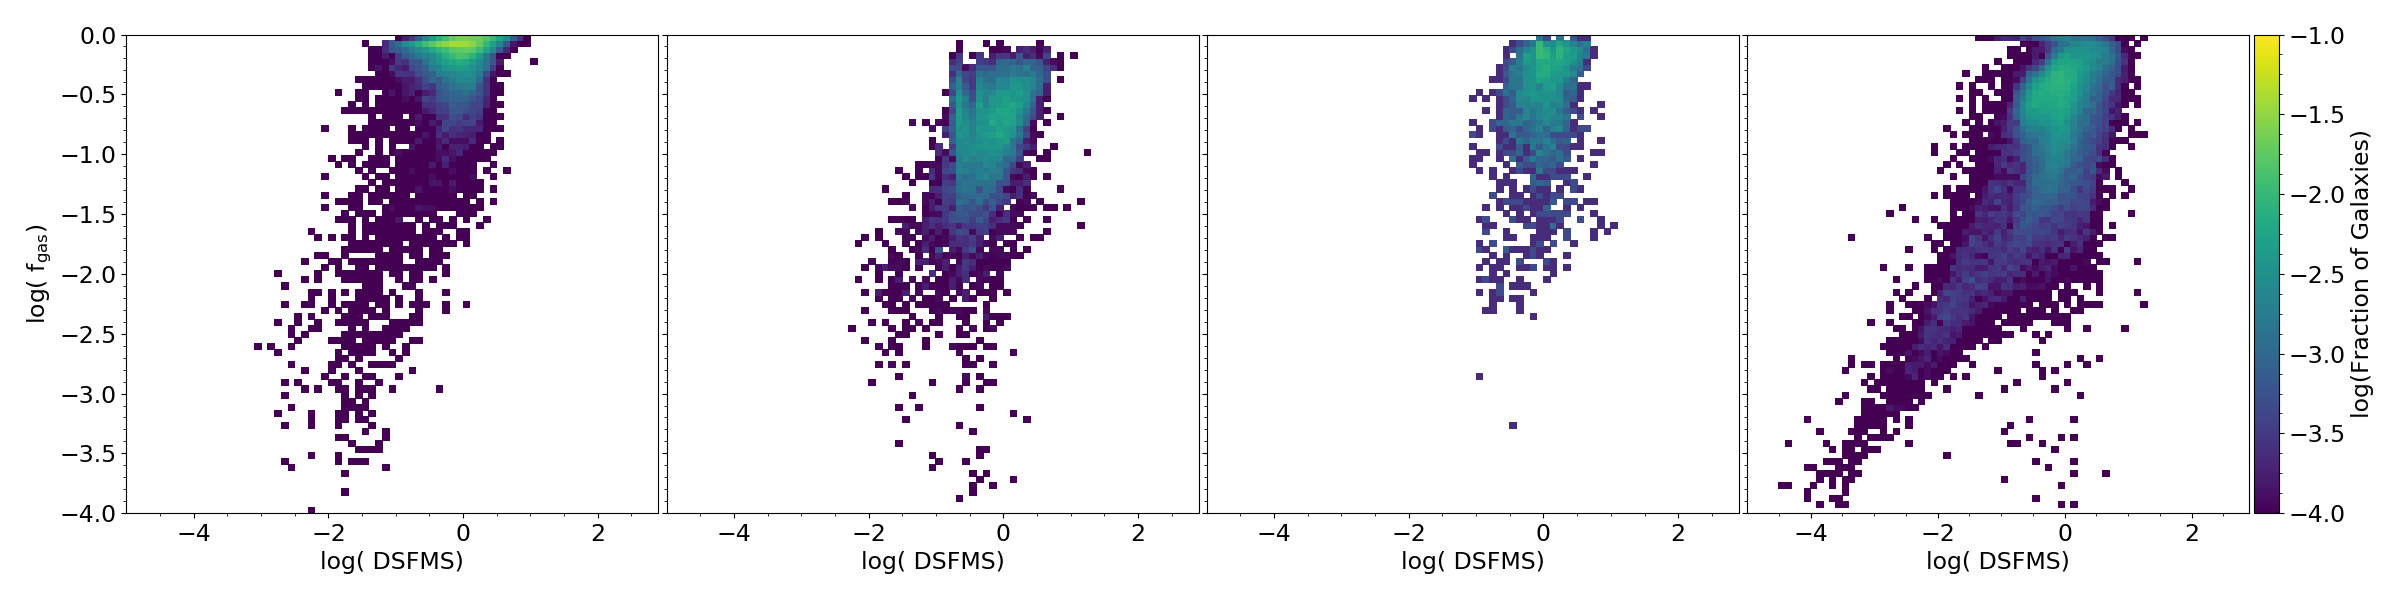
\includegraphics[width = 0.99\linewidth]{fgas_DSFMS_2dhist_count_log_fgas.png}\\
\caption{2D histogram of fraction of galaxies in a given gas fraction and distance from SFMS bin.}
\label{fig:fgas DSFMS panel}
\end{figure*}

\begin{figure*}
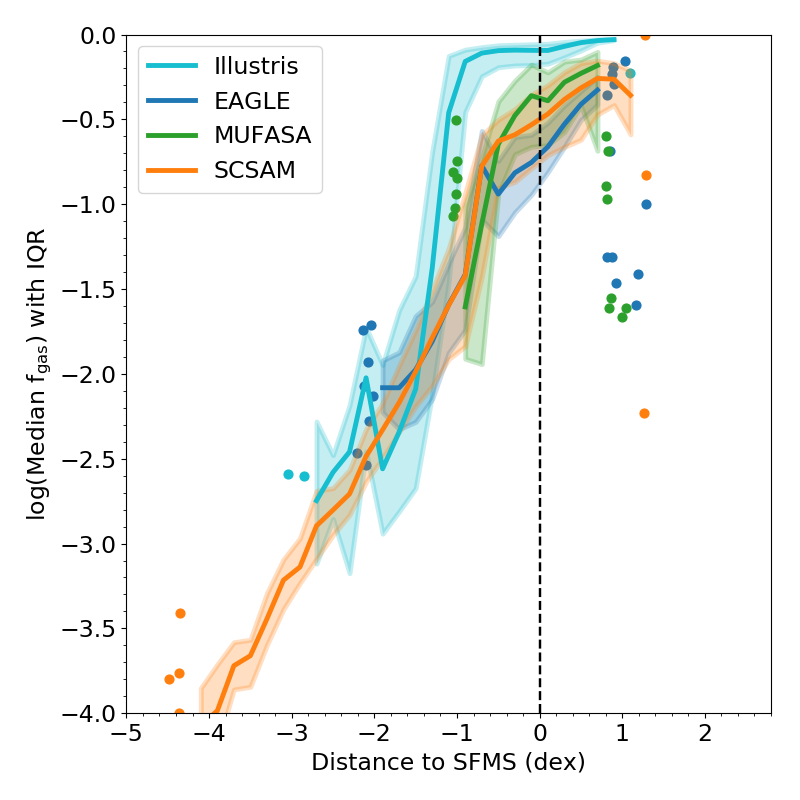
\includegraphics[width = 0.99\linewidth]{fgas_DSFMS_binned_IQR_logged.png}\\
\caption{Running median and IQR of the gas fraction of galaxies as a function of their distance (in dex) from the SFMS, as defined in Figure~\ref{fig:SFMS fgas}.}
\label{fig:fgas DSFMS}
\end{figure*}

\begin{figure*}
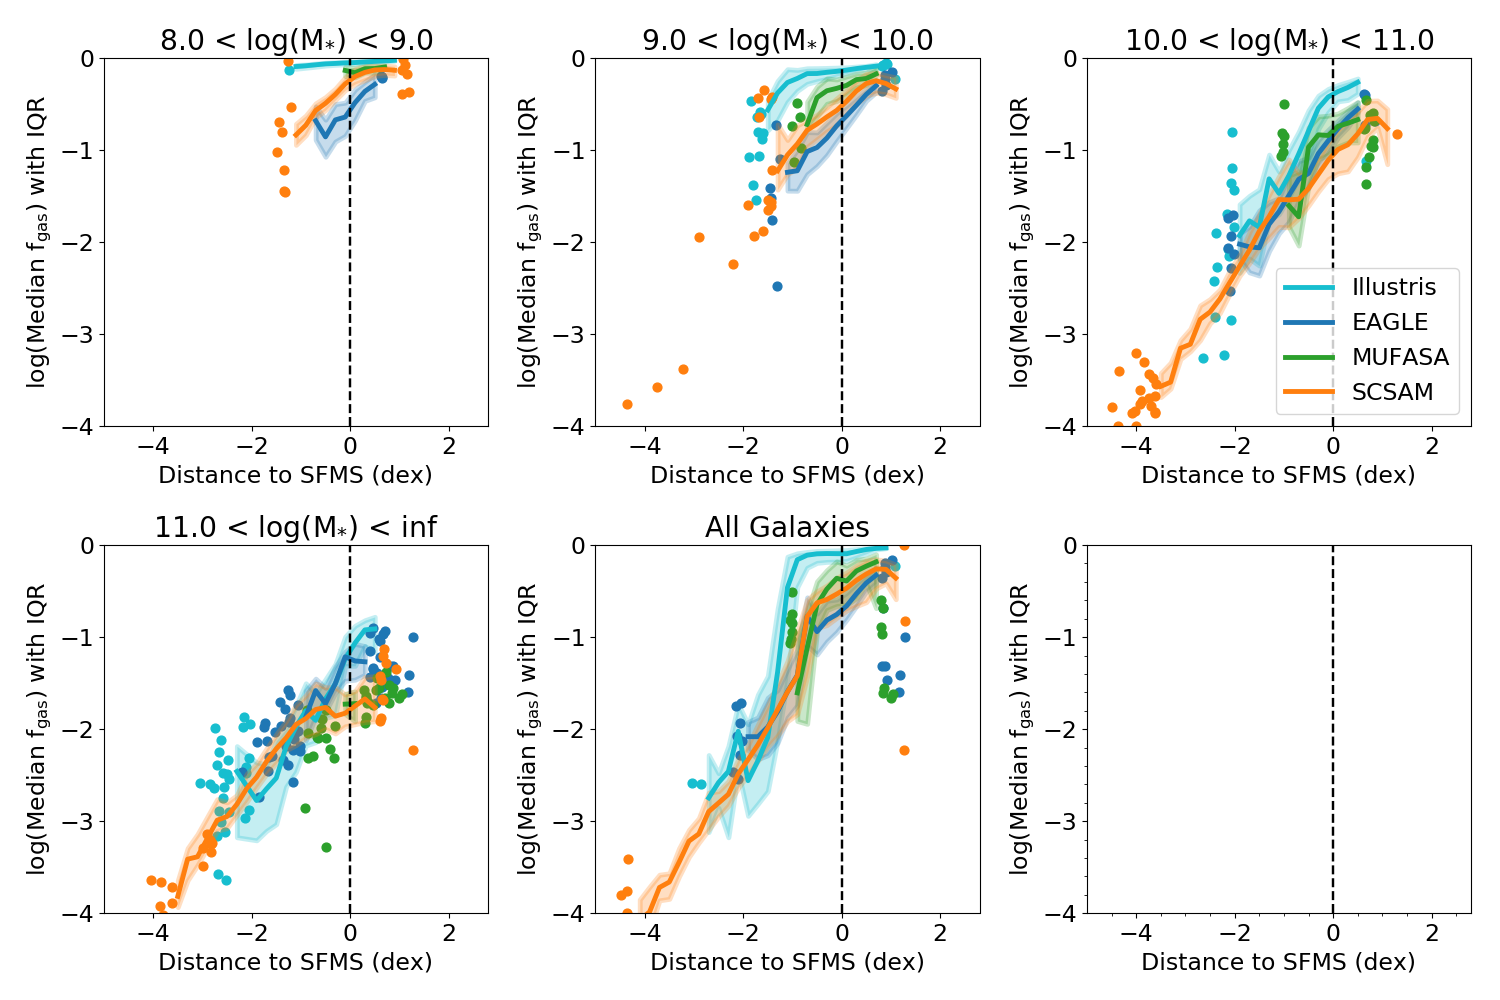
\includegraphics[width = 0.99\linewidth]{fgas_DSFMS_panel_plot_IQR_logged.png}\\
\caption{Same as Figure~\ref{fig:fgas DSFMS}, but separated into stellar mass bins.}
\label{fig:fgas DSFMS panel}
\end{figure*}

\begin{figure*}
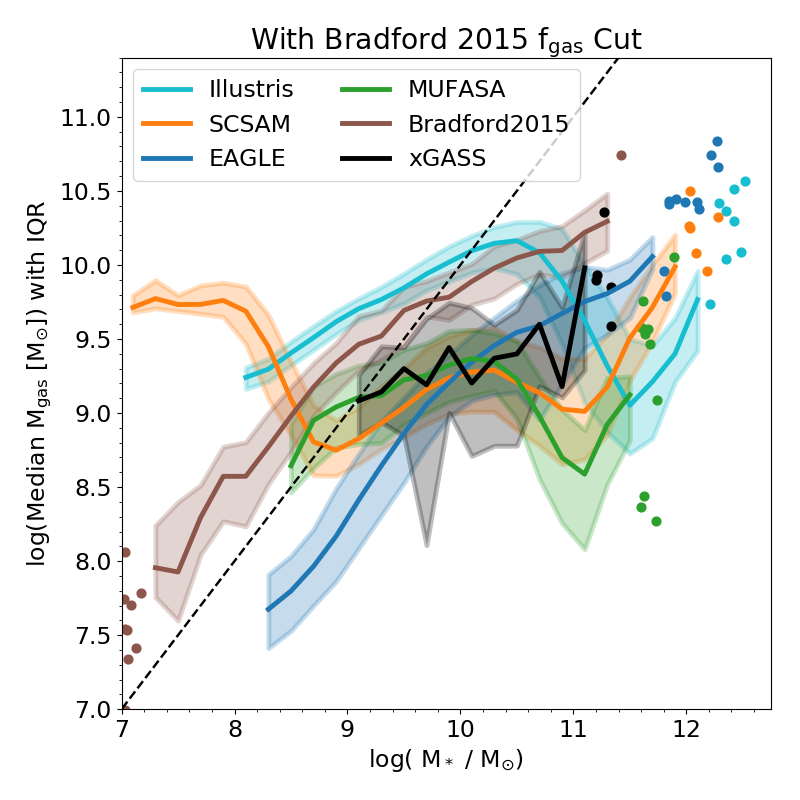
\includegraphics[width = 0.49\linewidth]{MHI_Mstar_binned_IQR_bradford_fgas_cut}
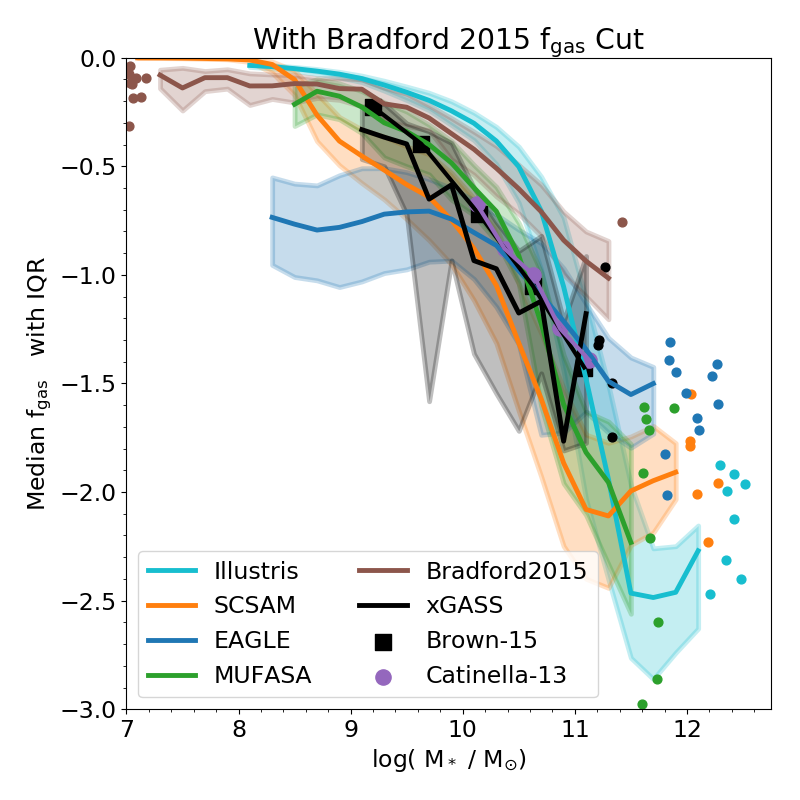
\includegraphics[width=0.49\linewidth]{fgas_mstar_binned_IQR_logged_bradford_fgas_cut.png}
\caption{Running medians of simulated galaxies in comparison to isolated galaxies from Bradford et. al. 2015 and the xGASS survey. The same Bradford et. al. 2015 limiting gas fraction thresholds were applied to all plotted data.}
\label{fig:fgas DSFMS panel}
\end{figure*}

\section{Discussion}

\subsection{Comparison to Observations}
\label{sec:observations}
{\it Possibly should not be the focal point of this paper, but could be nice to include. } 

\begin{figure*}
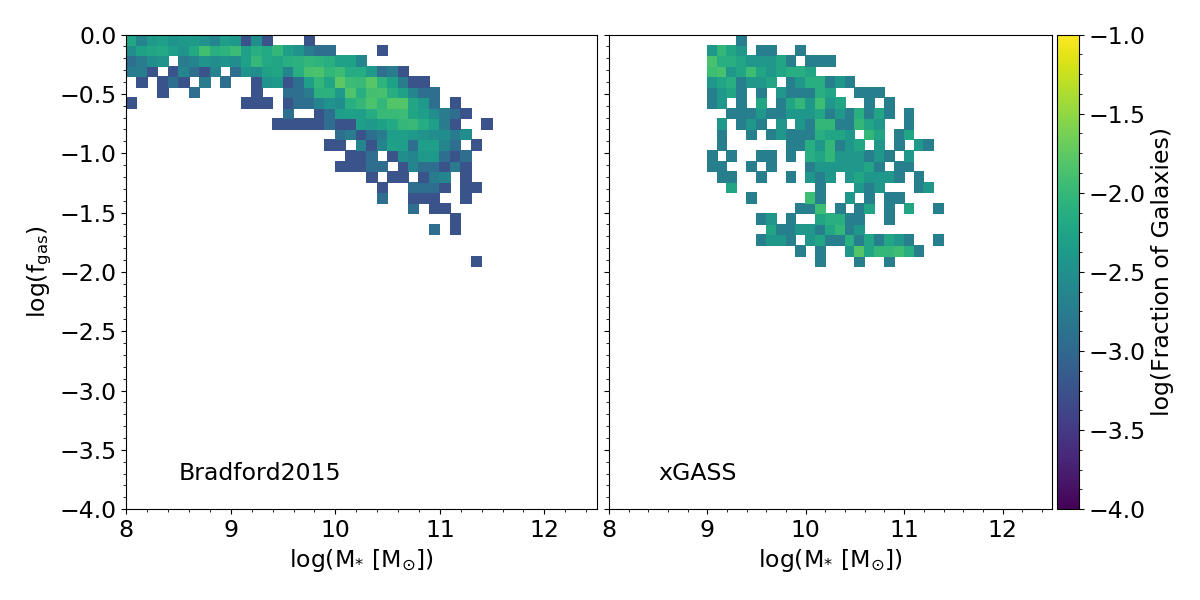
\includegraphics[width = 0.99\textwidth]{fgas_mstar_2D_log_fgas_obs.png}
\caption{Same as Figure~\ref{fig:fgas mstar 2D}, but for the observational data from Bradford2015 and Cantinella2018.}
\label{fig:fgas mstar 2D obs}
\end{figure*}

\begin{figure*}
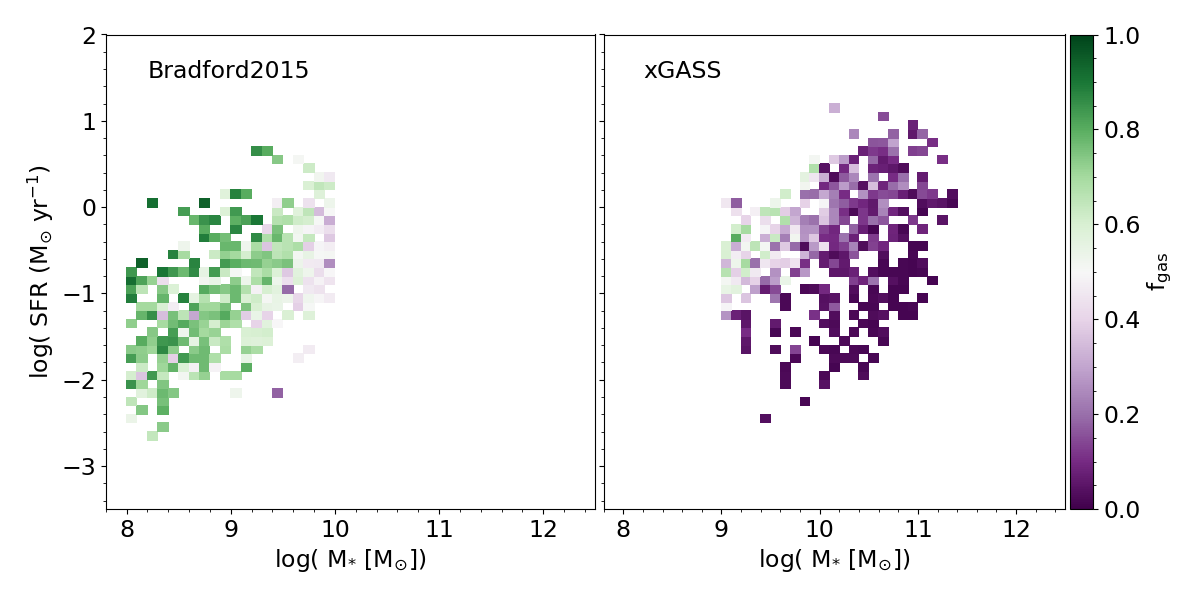
\includegraphics[width = 0.99\textwidth]{SFMS_fits_2dhist_median_obs.png}
\caption{Same as Figure~\ref{fig:SFMS fgas}, but for the observational data from Bradford2015 and Cantinella2018.}
\label{fig:SFMS mstar 2D obs}
\end{figure*}

\section{Conclusion}


\section*{Acknowledgements}
IQ collab and funding

%%%%%%%%%%%%%%%%%%%%%%%%%%%%%%%%%%%%%%%%%%%%%%%%%%

%%%%%%%%%%%%%%%%%%%% REFERENCES %%%%%%%%%%%%%%%%%%

% The best way to enter references is to use BibTeX:

\bibliographystyle{mnras}
\bibliography{msbib.bib} % if your bibtex file is called example.bib


% Alternatively you could enter them by hand, like this:
% This method is tedious and prone to error if you have lots of references

%%%%%%%%%%%%%%%%%%%%%%%%%%%%%%%%%%%%%%%%%%%%%%%%%%

%%%%%%%%%%%%%%%%% APPENDICES %%%%%%%%%%%%%%%%%%%%%


%%%%%%%%%%%%%%%%%%%%%%%%%%%%%%%%%%%%%%%%%%%%%%%%%%


% Don't change these lines
\bsp	% typesetting comment
\label{lastpage}
\end{document}

% End of mnras_template.tex